
\documentclass[11pt, oneside]{article} 
\usepackage{amsmath, amsthm, amssymb, wasysym, verbatim, bbm, color, geometry}
\usepackage{amsfonts}
\usepackage{csquotes}
\usepackage{polski}
% \usepackage[english]{babel}
\usepackage[nottoc]{tocbibind}
\usepackage{caption}
\usepackage{subcaption}
\usepackage{float}
\usepackage{graphicx}
\usepackage{circuitikz}
% \ctikzset{current arrow scale=1.5} 
\usepackage{hyperref} % Loads the hyperref package for hyperlinks
\usepackage{enumitem}
\usepackage{tikz}
\usepackage{pgfplots}
\usepackage[utf8]{inputenc}

\pgfplotsset{compat=1.18} % Set the compatibility level for pg
\usetikzlibrary{shapes.geometric, arrows, positioning, fit, backgrounds}

\hypersetup{
    colorlinks=true,
    linkcolor=blue,
    citecolor=cyan,
    urlcolor=blue!60,
    breaklinks=true,
}





\newcommand{\workSource}[2]{Tekst dostępny na stronie: \href{#1}{#2}}



\DeclareMathSizes{12}{12}{10}{8}
\makeatletter
\renewcommand\normalsize{%
\@setfontsize\normalsize{12pt}{13.5pt}% Will look incredibly crabbed if line height is too small
\abovedisplayskip 10\p@ \@plus2\p@ \@minus5\p@%
\abovedisplayshortskip \z@ \@plus2\p@%
\belowdisplayshortskip 5\p@ \@plus2\p@ \@minus3\p@%
\belowdisplayskip \abovedisplayskip%
\let\@listi\@listI%
}
\normalsize  
\makeatother

\newcommand{\der}{{\rm d}}
\newcommand{\R}{\mathcal{R}}
\newcommand{\C}{\mathcal{C}}
\newcommand{\M}{\mathcal{M}}
\newcommand{\G}{\mathcal{G}}
\newcommand{\Ron}{R_{\rm ON}}
\newcommand{\Roff}{R_{\rm OFF}}
\newcommand{\von}{V_{\rm ON}}
\newcommand{\voff}{V_{\rm OFF}}
\newcommand{\q}{q}
\newcommand{\ua}{v}
\newcommand{\ia}{i}
\newcommand{\phia}{\varphi}
\newcommand{\xw}{x}
\newcommand{\dert}[1]{\frac{{\rm d} {#1}}{{\rm d} t} }
\newcommand{\inv}[1]{\frac{1}{#1} }
\newcommand{\equal}{=}


\usepackage[style=numeric, 
            backend=biber,
           ]{biblatex}
           
\addbibresource{bibliography.bib} % Replace with your .bib file name

\geometry{tmargin=.75in, bmargin=.75in, lmargin=.75in, rmargin = .75in}  

% \usepackage{fontspec}
% \setmainfont[]{Palatino}

\newcommand{\Cdot}{\boldsymbol{\cdot}}

\newtheorem{thm}{Theorem}
\newtheorem{defn}{Definition}
\newtheorem{conv}{Convention}
\newtheorem{rem}{Remark}
\newtheorem{lem}{Lemma}
\newtheorem{cor}{Corollary}


\title{Modelowanie memrystorów SDC za pomocą sztucznych sieci neuronowych}
\author{Karol Bednarz}
\date{Rok akademicki 2024--2025}

\begin{document}

\maketitle
\tableofcontents

\vspace{.25in}

\newcommand{\Todo}[1]{\textcolor{red}{\textbf{TODO:} #1}}

\section{Wstęp}


W naukowej literaturze pojawiło się wiele modeli memrystorów po odkryciu ich zachowań memrystywnych na nanoskalę. Oryginalny model, zaproponowany w \cite{Strukov2008}, konceptualizuje memrystor jako połączenie szeregowe dwóch zmiennych rezystancji odpowiadających warstwom przewodzącym i izolacyjnym filmu. W celu lepszego modelowania memrystorów SDC (ang. Self-Directed Channel), M. Nugent i T. Molter zaproponowali uogólniony model Mean Metastable Switch, który jest modelem półempirycznym. Pochodna zmiennej stanu jest tu określana jako funkcja prawdopodobieństw przejścia do kolejnych stanów i aktualnej wartości zmiennej stanu~\cite{Molter2016}. W pracy~\cite{Lee2024} autorzy podjęli próbę modelowania memrystora z wykorzystaniem podejścia opartych na Physics-Informed Neural Networks (PINNs). Mimo że przedstawione tam wyniki wskazują na potencjał tej metody, badania nie opierają się na rzeczywistych pomiarach fizycznych memrystorów, lecz jedynie na porównaniach z wynikami uzyskanymi z istniejących modeli symulacyjnych. Co więcej, dane treningowe użyte w procesie uczenia sieci neuronowej zostały wygenerowane na podstawie wcześniej opracowanych matematycznych modeli teoretycznych, co ogranicza możliwość weryfikacji skuteczności podejścia w kontekście rzeczywistych układów fizycznych.

W pracy \cite{Ricky2018} autorzy przedstawiają koncepcję głębokich modeli neuronowych, w których dynamika ukrytego stanu opisywana jest za pomocą równania różniczkowego zwyczajnego (ODE, ang. Ordinary Differential Equation). Uczenie modelu przebiega w sposób end-to-end, co oznacza optymalizację wszystkich parametrów jednocześnie w ramach jednego procesu treningowego. Kluczowym elementem proponowanego podejścia jest nowa metoda propagacji wstecznej błędu, oparta na rozwiązywaniu równania różniczkowego wstecz w czasie z wykorzystaniem metod sprzężonych (ang. adjoint methods). Rozwiązanie to znajduje zastosowanie m.in. w ciągłych odpowiednikach sieci rezydualnych (continuous-depth residual networks) oraz generatywnych modelach przepływowych (generative flow-based models).

Z kolei praca \cite{Ricky2021} rozszerza klasyczne modele Neural ODE, umożliwiając modelowanie nieciągłych zdarzeń w czasie ciągłym — bez uprzedniej wiedzy na temat ich liczby ani momentu wystąpienia. Wprowadzone przez autorów różniczkowalne funkcje zdarzeń pozwalają na efektywną symulację systemów hybrydowych, takich jak układy z kolizjami, przełącznikami stanów czy procesami punktowymi, co otwiera nowe możliwości w zakresie modelowania i trenowania układów z dyskretnym sterowaniem.

\Todo{Dodać więcej informacji o pracy, w tym o zastosowaniach i wynikach.}

Niniejsza praca ma na celu zbadanie możliwości modelowania memrystorów SDC przy użyciu sztucznych sieci neuronowych, oraz porównanie skuteczności tego podejścia z istniejącymi modelami teoretycznymi. W szczególności, skupimy się na zastosowaniu modeli Neural ODE do symulacji zachowania memrystorów SDC, wykorzystując dane eksperymentalne uzyskane z rzeczywistych układów fizycznych. Naszym celem jest ocena, czy modele oparte na sztucznych sieciach neuronowych mogą skutecznie odwzorować dynamikę memrystorów SDC i czy oferują przewagę w porównaniu do tradycyjnych modeli teoretycznych.

\section{Materiały i metody}

\subsection{Memrystory, oraz pomiary}
W niniejszej pracy wykorzystano dane eksperymentalne pozyskane z rzeczywistych memrystorów typu SDC (ang. Self Directed Channels) domieszkowanych wolframem. Struktura oraz właściwości tych elementów zostały szczegółowo opisane w literaturze, m.in. w~\cite{Garda2024, Campbell2017}. Pomiary przeprowadzono na układzie przedstawionym na Rys.~\ref{fig:memristor_setup}, który składa się z memrystora połączonego szeregowo z rezystorem. Napięcie zasilania było generowane przez generator arbitralny, a pomiary  napięcia były dokonywane za karty pomiarowej. Pomiary zostały przeprowadzone dla różnych kombinacji częstotliwości oraz amplitud napięcia zasialania, gdzie amplituda niępiacia zasilania $V_s \in \{ 0.5, 1, 1.5 \} \mathrm{[V]}$ oraz częstotliwość $f \in \{ 1, 5, 10, 20, 50, 100 \} \ {\rm [Hz]}$.

\begin{figure}[H]
    \centering
    \resizebox{0.5\linewidth}{!}{%
        
\begin{circuitikz}[american, cute inductors, transform shape]
  \draw (0, 0)
  to [vsourcesin, fill=blue, l=\(v_s \equal V_s\sin (2 \pi f_s \cdot t)\)] (1,0)
  to  [memristor, fill=yellow, l=\(M\), v=\(v_{m}\), invert] (4,0)
  to [short, i=\(i_{m}\)] (4.5,0)
  to [R, l=\(R_s\), v=\(v_{r}\)] (6.5,0);
  \draw (0,0) -- (-0.5,0) node[rground]{};
  \draw (6.5,0) -- (7,0) node[rground]{};
  \draw (0,-2.5);
\end{circuitikz}}
    \vspace{-0.5in}
    \caption{Schemat układu pomiarowego memrystora SDC.}
    \label{fig:memristor_setup}
\end{figure}

\subsection{Modelowanie za pomocą sieci neuronowej}

Analizowany model opiera się na ogólnym opisie elementu memrystywnego, wyrażonym za pomocą równań \eqref{eq:memristor_model1}, \eqref{eq:memristor_model}
\begin{align}
    \label{eq:memristor_model1}
    \ua(t)                  & = \M \Big(\xw(t),\ua(t)\Big) \ia(t), \\
    \label{eq:memristor_model}
    \frac{\der \xw}{\der t} & = f\Big(\xw(t),\ua(t)\Big)
\end{align}
gdzie $\xw \in \langle 0, 1 \rangle$ oznacza wewnętrzną zmienną stanu, której ewolucja przebiega zgodnie z określoną dynamiką $f$, natomiast $\M$ reprezentuje memrystancję urządzenia. Kluczowym zagadnieniem modelowania memrystora jest odpowiednie wyznaczenie funkcji $\M(\xw, \ua)$ oraz $f(\xw, \ua)$.

W przeprowadzonych badaniach przyjęto powszechnie stosowaną postać funkcji memrystancji:
\begin{equation}
    \M(x) = x \Ron + (1-x) \Roff,
\end{equation}
gdzie $\Ron$ oraz $\Roff$ odpowiadają wartościom rezystancji w stanach niskiej i wysokiej przewodności. Funkcja $f(\xw(t), \ua(t))$ została zaimplementowana w postaci sztucznej sieci neuronowej, której ideowa architektura przedstawiona została na Rys.~\ref{fig:nn_structure}. W trakcie procesu optymalizacji sieci, równocześnie dostrajane są jej parametry (wagi i biasy) oraz wartości $\Ron$ i $\Roff$.

\begin{figure}[H]
    \centering
    \includegraphics[width=0.5\textwidth]{figs/Rysowanie_schematów.pdf}
    \caption{Diagram ideowy zastosowania sieci neuronowej do symulacji dynamiki memrystora.}
    \label{fig:nn_structure}
\end{figure}

\subsection{Model MMS - Mean Metastable Switch}
W celu porównania skuteczności modelu, porównano go z deterministycznym modelem Mean Metastable Switch (MMS) zaproponowanym w pracach \cite{Molter2016, Ostrovskii2021}. Model ten opisuje dynamikę memrystora za pomocą równań \eqref{eq:mms}, \eqref{eq:beta}.

\begin{align}
    \label{eq:mms}
    \dert{x} & =  \frac{1}{\tau} \Bigg( \frac{1}{1+e^{-\beta \big(\ua(t)-\von\big)}} (1-x)  -\Bigg(1- \frac{1}{1+e^{-\beta \big(\ua(t)-\voff\big)}} \Bigg) x \Bigg) \\
    \label{eq:beta}
    \beta    & = \frac{q}{kT}
\end{align}
gdzie, $\beta$ jest parametrem temperaturowym, $\von$ napięciem przełączania w stan LRS, $\voff$ napięciem przełączania w stan HRS, $k$ stałą Boltzmanna, $T$ temperaturą,  $q$ ładunkiem elementarnym.

Chwilowa konduktancja memrystora jest określona jako:
\begin{equation}
    \G_{m}(\xw) = \frac{\xw}{R_{\rm ON}}+\frac{1-\xw}{R_{\rm OFF}}
\end{equation}

Gdzie $\Ron$ odpowiada rezystancji w stanie LRS, a $\Roff$ rezystancji w stanie HRS.
Inne funkcje opisywane w literaturze, to między innymi:
\begin{itemize}
    \item $\G_m(x) = (x R_{\mathrm{ON}} + (1-x) R_{\mathrm{OFF}})^{-1}$
    \item $\G_m(x) = \frac{1}{R_{\mathrm{ON}}} \left( \frac{R_{\mathrm{OFF}}}{R_{\mathrm{ON}}} \right)^{x-1}$
\end{itemize}
Wpływ tych funkcji na rezystancje został przedstawiony na Rys.~\ref{fig:m-x}.
\begin{figure}[H]
    \centering
    \resizebox{0.5\linewidth}{!}{%
        
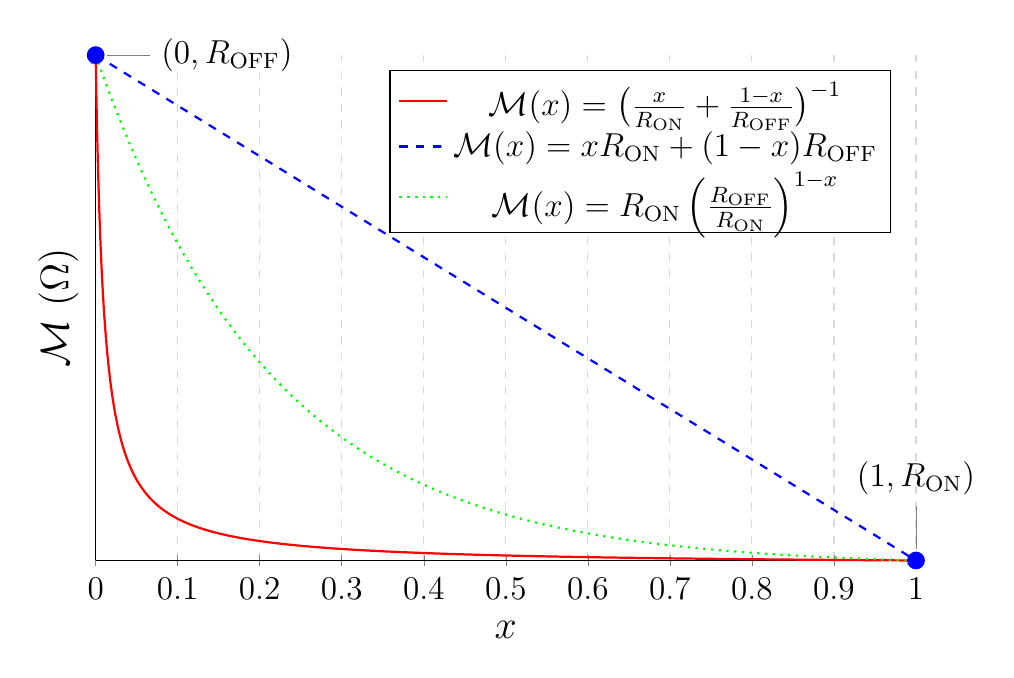
\begin{tikzpicture}
  \begin{axis}[
      width=12cm,
      height=8cm,
      xlabel={$x$},
      ylabel={ $\M$ ($\Omega$)},
      grid=major,
      grid style={dashed, gray!30},
      % xmin=0, xmax=1,
      % ymin=0, ymax=12,
      legend pos=north east,
      axis lines=left,
      tick label style={font=\normalsize},
      label style={font=\Large},
      title style={font=\Large\bfseries},
      ytick=\empty,
      clip=false
    ]

    % Define parameters
    \pgfmathsetmacro{\RON}{100}     % R_ON in ohms
    \pgfmathsetmacro{\ROFF}{10000}  % R_OFF in ohms

    % Plot the function G_m(w) = w/R_ON + (1-w)/R_OFF
    \addplot[
      domain=0:1,
      samples=1000,
      thick,
      red,
      smooth
    ] {1/(x/\RON + (1-x)/\ROFF)};


    \addlegendentry{$\M(x) = \big(\frac{x}{R_{\mathrm{ON}}} + \frac{1-x}{R_{\mathrm{OFF}}}\big)^{-1}$}

    \addplot[
      domain=0:1,
      samples=1000,
      thick,
      blue,
      smooth,
      dashed
    ] {x*\RON + (1-x)*\ROFF};


    \addlegendentry{$\M(x) = x R_{\mathrm{ON}} + (1-x) R_{\mathrm{OFF}}$}



    \addplot[
      domain=0:1,
      samples=1000,
      thick,
      green,
      smooth,
      dotted
    ] {\RON * (\ROFF/\RON)^(1-x)};

    \addlegendentry{$\M(x) = R_{\mathrm{ON}} \left( \frac{R_{\mathrm{OFF}}}{R_{\mathrm{ON}}} \right)^{1-x}$}




    % Add parameter annotations
    % \node[anchor=north west] at (axis cs:0.05,11) {
    %   \begin{tabular}{l}
    %     $R_{\mathrm{ON}} = 100\,\Omega$ \\
    %     $R_{\mathrm{OFF}} = 10000\,\Omega$
    %   \end{tabular}
    % };

    % Mark key points
    \addplot[only marks, mark=*, mark size=3pt, blue] coordinates {(0, {\ROFF}) (1, {\RON})};

    % Add labels for key points
    \node[pin=-0:{$(0, R_{\mathrm{OFF}})$}] at (axis cs:0,{\ROFF}) {};
    \node[pin=90:{$(1, R_{\mathrm{ON}})$}] at (axis cs:1,{\RON}) {};

  \end{axis}
\end{tikzpicture}
    }
    \caption{Porównanie funcki rezystancji $R_m(x)$ dla różnych modeli memrystora.}
    \label{fig:m-x}
\end{figure}


W pracy \cite{Molter2016} autorzy również model GMMS (Generalized Mean Metastable Switch), który opisuje memrystor jako równoległe połączenie dwóch memrystora wraz z diodą Schottky'ego. Model ten jest bardziej złożony i uwzględnia nieliniowość charakterystyki prądowo-napięciowej, co pozwala na lepsze odwzorowanie rzeczywistych zachowań memrystora w różnych warunkach pracy.Wprowadzone jednak dodatkowe parametry oraz nieliniowość sprawiają, że model ten jest bardziej skomplikowany i trudniejszy do optymalizacji. Pochodna zmiennej stanu koresponduje z rów. \eqref{eq:mms}, jednak zależność prądowo napięciowa jest opisana równaniami:

\begin{align}
    i(t)      & = \phi i_m(v, t) + (1-\phi) i_d(v)                 \\
    i_d(v)    & = \alpha_f e^{\beta_f v} - \alpha_r e^{-\beta_r v} \\
    i_m(v, t) & = \G_m(x) v
\end{align}

gdzie $\phi \in [0,1]$, jest to parametr określający udział prądu płynącego przez memrystor w całkowitym prądzie płynącym przez element. Parametry $\alpha_f$, $\beta_f$, $\alpha_r$ oraz $\beta_r$ są parametrami dodatnimi, które określają zachowanie prądów w kierunku przewodzenia i zaporowym, wzdłuż bariery Schottky'ego.

W przypadku modelu GMMS, wyzwaniem jest również, ze względu na efekt Schottky'ego, konieczność uwzględnienia nieliniowości charakterystyki prądowo-napięciowej, co przy szeregowym połaczeniu memrystora z rezystorem, daje konieczność rozwiązania numerycznie nieliniowego równania w postaci:
\begin{equation}
    v_s(t) = v_r(t) + v_m(t)
\end{equation}
gdzie, $v_s(t)$ to napięcie zasilania, $v_r(t) = R_s i(t)$ to napięcie na rezystorze, a $v_m(t)$ to napięcie na memrystorze, czyni to jednak układ sztywnym, oraz nie pozwala na automatyczne różniczkowanie względem parametrów, dla funckji celu. Drugą metodą jest zastosowanie różniczkowania implikowanego.
Niech $F$ będzie funkcją określoną równaniem:
\begin{equation}
    F(v_m, t) = v_s(t) - v_r(v_m, t) - v_m(t) = 0
\end{equation}
Korzystając z regułu łańcuchowej:
\begin{equation}
    \frac{\der F}{\der t} = \frac{\partial F}{\partial v} \frac{\der v}{\der t} + \frac{\partial F}{\partial t} = 0
\end{equation}
Zatem:
\begin{equation}
    \frac{\der v}{\der t} = -\frac{\partial F / \partial t}{\partial F / \partial v}
\end{equation}
Podstawiajac równania:
\begin{equation}
    \frac{\der v_m}{\der t} = - \frac{\der v_s}{\der t}\frac{1}{- R_s \left(\G_{m} \phi + \left(1 - \phi\right) \left(\alpha_f \beta_f e^{\beta_f v_m} + \alpha_r \beta_r e^{- \beta_r v_m}\right)\right) - 1}
\end{equation}

Tak więc układ wymaga dodatkowej zmiennej stanu, lecz nie jest konieczne rozwiązywanie nieliniowego układu równań z każdym krokiem czasowym. Tak więc układ równań opsisujący ukłąd memrystora z rezystorem, przy zastosowaniu modelu GMMS, jest następujący:

\begin{equation}
    \left\{
    \begin{aligned}
         & \dert{x} = \frac{1}{\tau} \Bigg( \frac{1}{1+e^{-\beta \big(v_m(t)-\von\big)}} (1-x)  -\Bigg(1- \frac{1}{1+e^{-\beta \big(v_m(t)-\voff\big)}} \Bigg) x \Bigg)                                            \\
         & \frac{\der v_m}{\der t} = \frac{\der v_s}{\der t}\frac{1}{ R_s \left(\G_{m} \phi + \left(1 - \phi\right) \left(\alpha_f \beta_f e^{\beta_f v_m} + \alpha_r \beta_r e^{- \beta_r v_m}\right)\right) - 1}
    \end{aligned}
    \right.
\end{equation}


\subsection{Funkcja celu}

Funkcja straty oparta na portrecie fazowym została zaprojektowana w taki sposób, aby jednocześnie uwzględniać zarówno wielkości bezwzględne sygnału, jak i jego strukturę dynamiczną. W tym celu definiuje się ją jako sumę czterech składników, z których każdy pełni odmienną, komplementarną rolę w procesie optymalizacji. Całkowita funkcja straty przyjmuje postać, jak w równaniu~\eqref{eq:loss_function}:

\begin{equation}
    \mathcal{L}_{\mathrm{total}} = \mathcal{L}_{\mathrm{base}} + \lambda_1 \cdot \mathcal{L}_{v} + \lambda_2 \cdot \mathcal{L}_{c} + \lambda_{\mathrm{con}} \cdot\mathcal{L}_{\rm con}(x)
    \label{eq:loss_function}
\end{equation}
gdzie $\mathcal{L}_{\mathrm{base}}$ stanowi podstawowy składnik błędu, zazwyczaj odnoszący się do różnicy między wartościami przewidywanymi a referencyjnymi (np. błąd średniokwadratowy – MSE), $\mathcal{L}_{v}$ odpowiada za zachowanie poprawnej charakterystyki prędkości zmian, tj. pochodnych trajektorii w przestrzeni fazowej, $\mathcal{L}_{c}$ odpowiada za zgodność trajektorii w kontekście zakrzywień (np. poprzez analizę krzywizny lub zmian kierunku trajektorii), $\mathcal{L}_{\mathrm{con}}(x)$ wprowadza dodatkowe ograniczenia fizyczne lub strukturalne, które powinny być spełnione przez model, np. warunki stabilności, nieliniowości bądź zgodności z modelem fizycznym.
Współczynniki wagowe $\lambda_1$, $\lambda_2$ oraz $\lambda_{\mathrm{con}}$ służą do odpowiedniego zbalansowania wkładu poszczególnych składników w całkowitej funkcji straty, w zależności od priorytetów modelowania. Tak skonstruowana funkcja pozwala na lepsze odwzorowanie zarówno ilościowych, jak i jakościowych aspektów dynamiki badanego systemu.


Dla trajektorii obwodu oznaczonych indeksem \( k = 1, \ldots, N_{\text{traj}} \), każda zmienna \( z \in \{v, i\} \), reprezentująca odpowiednio napięcie lub prąd, jest normalizowana względem odchylenia standardowego wyznaczonego osobno dla każdej trajektorii:
\begin{equation}
    \sigma_{z,k} = \sqrt{\frac{1}{T-1} \sum_{t=1}^{T} \left(z_{k,t}^{\mathrm{true}} - \bar{z}_k^{\mathrm{true}}\right)^2}
\end{equation}
gdzie średnia trajektorii wynosi:
\begin{equation}
    \bar{z}_k^{\mathrm{true}} = \frac{1}{T} \sum_{t=1}^{T} z_{k,t}^{\mathrm{true}},
\end{equation}
a \( T \) oznacza długość danej trajektorii (liczbę punktów czasowych).

Tak przeprowadzona normalizacja zmiennych w obrębie każdej trajektorii pozwala na ujednolicenie skali sygnałów niezależnie od ich amplitudy, co ma istotne znaczenie w kontekście porównywania dynamicznych kształtów przebiegów oraz zapewnienia stabilności procesu uczenia.

Podstawowy składnik funkcji straty odpowiada za dopasowanie modelu do rzeczywistych danych napięciowo-prądowych, przy uwzględnieniu normalizacji względem trajektorii. Ma on na celu minimalizację błędu średniokwadratowego (MSE) między przewidywanymi a rzeczywistymi przebiegami napięcia i prądu, znormalizowanymi względem odchylenia standardowego każdej trajektorii. Formalnie wyraża się to jako:
\begin{equation*}
    \mathcal{L}_{\mathrm{base}} = \frac{1}{N_{\text{traj}}} \sum_{k=1}^{N_{\text{traj}}} \left[\mathrm{MSE}\left(\frac{v_{\mathrm{pred},k}}{\sigma_{v,k}}, \frac{v_{\mathrm{true},k}}{\sigma_{v,k}}\right) +  \mathrm{MSE}\left(\frac{i_{\mathrm{pred},k}}{\sigma_{i,k}}, \frac{i_{\mathrm{true},k}}{\sigma_{i,k}}\right)\right]
\end{equation*}

Porównanie dynamiki pierwszego rzędu pozwala na ocenę zgodności prędkości zmian napięcia i prądu między przewidywaniami modelu a rzeczywistymi danymi, zwłaszcza w kontekście szybkiego przełączania stanów memrystora. Dzięki temu model jest uczony nie tylko na podstawie wartości bezwzględnych sygnałów, ale również ich tempa zmian, co jest szczególnie istotne w przypadku systemów dynamicznych. Jest definiowany jako:

\begin{equation}
    \mathcal{L}_{v} = \mathrm{MSE}\left(\dert{v}_{\mathrm{pred}}, \dert{v}_{\mathrm{true}}\right) + \mathrm{MSE}\left(\dert{i}_{\mathrm{pred}}, \dert{i}_{\mathrm{true}}\right)
\end{equation}


Porównanie drugiego rzędu, czyli krzywizny trajektorii, jest kluczowe dla uchwycenia subtelnych zmian w dynamice systemu, które mogą być istotne w kontekście nieliniowych zachowań memrystora. Składnik ten pozwala na lepsze odwzorowanie właściwości krzywizny trajektorii w przestrzeni fazowej, co jest istotne przy modelowaniu systemów nieliniowych i silnie dynamicznych. Jest definiowany jako:
\begin{equation}
    \mathcal{L}_{c} = \mathrm{MSE}\left(\frac{\mathrm{d}^2v}{\mathrm{d}t^2}_{\mathrm{pred}}, \frac{\mathrm{d}^2v}{\mathrm{d}t^2}_{\mathrm{true}}\right)
\end{equation}

W celu wymuszenia przynależności wartości parametrów do określonych przedziałów zastosowano następującą funkcję kosztu:

\begin{equation}
    \mathcal{L}_{\mathrm{con}}(\mathbf{x}) =  \mathbb{E}\left[\left(
        \sigma\left(-\frac{\mathbf{x} - (a + \delta)}{\delta/4}\right) \cdot ((a + \delta) - \mathbf{x}) +
        \sigma\left(\frac{\mathbf{x} - (b - \delta)}{\delta/4}\right) \cdot (\mathbf{x} - (b - \delta))
        \right)^2\right]
\end{equation}
gdzie: $\sigma(z) = \frac{1}{1 + e^{-z}}$ oznacza funkcję sigmoidalną,
$a$ i $b$ oznaczają odpowiednio dolne i górne ograniczenie zakresu dopuszczalnych wartości parametru,
$\delta$ określa margines przejścia (szerokość strefy przejściowej między dopuszczalnym a karanym zakresem),
$\lambda_{\mathrm{con}}$ to współczynnik wagowy odpowiadający za siłę działania ograniczenia,
$\mathbb{E}$ oznacza wartość oczekiwaną (średnią po zbiorze parametrów lub trajektorii).

Podczas trenowania sieci neuronowej zastosowano następujące ograniczenia przedziałowe, aby zapewnić fizycznie sensowne i numerycznie stabilne wartości parametrów:
\begin{itemize}
    \item $R_{\mathrm{ON}} \in (0, 100)\,\ \mathrm{k}\Omega$ oraz $R_{\mathrm{OFF}} \in (0, 100)\,\mathrm{k}\Omega$ – w celu ograniczenia możliwych stanów rezystancyjnych,
    \item $x_0 \in (0, 1)$ – aby ograniczyć początkowy stan wewnętrzny do fizycznie dopuszczalnych wartości,
    \item $x(t) \in (0, 1)$ – w celu utrzymania zmiennej stanu wewnętrznego w znormalizowanej dziedzinie w trakcie całej symulacji.
\end{itemize}

Przykładowe działanie funkcji ograniczającej $\mathcal{L}_{\mathrm{con}}(\mathbf{x})$ przedstawiono na Rys.~\ref{fig:constrains}, dla wartości:  $a=0$, $b=1$, $\delta=0.01$ w zakresie $\mathbf{x} \in (-0.5, 1.5)$.

\begin{figure}[H]
    \centering
    \resizebox{0.5\linewidth}{!}{%
        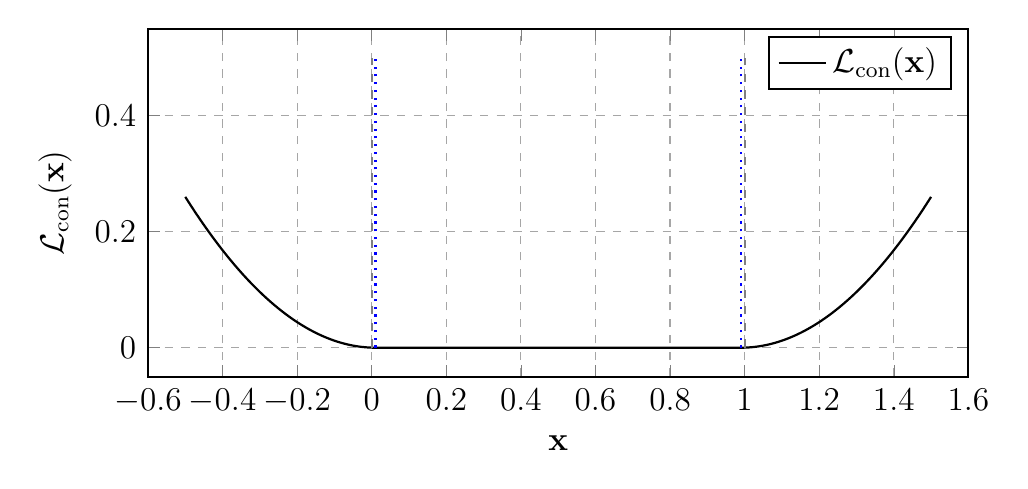
\begin{tikzpicture}
  \begin{axis}[
    width=12cm,
    height=6cm,
    xlabel={$\mathbf{x}$},
    ylabel={$\mathcal{L}_{\mathrm{con}}(\mathbf{x})$},
    grid=major,
    grid style={dashed,gray!70},
    legend style={at={(0.98,0.98)},anchor=north east},
    domain=-0.5:1.5,
    samples=500,
    thick,
    % Automatic spacing like matplotlib margins
    enlarge x limits=0.05,
    enlarge y limits=0.1,
    ]

    % Main function plot
    \addplot [
      color=black,
    ]
    {(1/(1 + exp(-(-((x - 0.01)/0.0025)))) * (0.01 - x)
      + 1/(1 + exp(-((x - 0.99)/0.0025))) * (x - 0.99))^2};
    \addlegendentry{$\mathcal{L}_{\mathrm{con}}(\mathbf{x})$}

    % Vertical reference lines using simple approach
    \addplot[dashed, gray, forget plot] coordinates {(0,0) (0,0.5)};
    \addlegendentry{$a = 0$}

    \addplot[dashed, gray, forget plot] coordinates {(1,0) (1,0.5)};
    \addlegendentry{$b = 1$}

    \addplot[dotted, blue, forget plot] coordinates {(0.01,0) (0.01,0.5)};
    \addlegendentry{$a + \delta$}

    \addplot[dotted, blue, forget plot] coordinates {(0.99,0) (0.99,0.5)};
    \addlegendentry{$b - \delta$}
  \end{axis}
\end{tikzpicture}
    }
    \caption{Przykładowe działanie funkcji ograniczającej $\mathcal{L}_{\mathrm{con}}(\mathbf{x})$ dla wartości:  $a=0$, $b=1$, $\delta=0.01$ w zakresie $\mathbf{x} \in (-0.5, 1.5)$.}
    \label{fig:constrains}
\end{figure}


\subsection{Detale implementacji}
Proces tworzenia oraz trenowania modelu sieci neuronowej został zrealizowany przy wykorzystaniu frameworka \texttt{PyTorch}, zaimplementowanego w języku \texttt{Python}.

W celu umożliwienia integracji równań różniczkowych w trakcie procesu uczenia, zastosowano bibliotekę \texttt{torchdiffeq}. Biblioteka ta udostępnia różniczkowalne rozwiązywacze równań różniczkowych zwyczajnych (ODE), co pozwala na efektywne wyliczanie gradientów względem trajektorii rozwiązania poprzez zastosowanie metody czułości sprzężonej (ang. adjoint sensitivity method). Dzięki temu możliwe jest przeprowadzenie end-to-end treningu modeli opisywanych dynamiką wyrażoną za pomocą równań różniczkowych. W szczególności wykorzystano solver \texttt{dopri5}. Architektura sieci neuronowej została przedstawiona na Rys.~\ref{fig:nn-arch}. Redukcja wymiaru w pierwszej i ostatniej warstwie ukrytej wynika z kilku istotnych aspektów:

\begin{itemize}
    \item Zmniejszenie liczby parametrów sieci, co przyczynia się do szybszego uczenia oraz redukcji ryzyka przeuczenia (overfitting).
    \item Efektywna ekstrakcja istotnych cech z danych wejściowych, co sprzyja poprawie zdolności modelu do generalizacji.
    \item Stabilizacja procesu uczenia poprzez ograniczenie liczby parametrów, co może prowadzić do bardziej stabilnej i szybszej konwergencji.
    \item Wprowadzenie mechanizmu regularyzacji za pomocą konstrukcji bottleneck, sprzyjającej wypracowaniu bardziej skoncentrowanej reprezentacji wewnętrznej, korzystnej dla modelowania dynamiki systemów.
    \item Redukcja ryzyka zaniku lub eksplozji gradientu, co ma szczególne znaczenie przy modelowaniu długich sekwencji czasowych.
\end{itemize}


Do optymalizacji wag sieci wykorzystano algorytm \texttt{Adam}, który jest jedną z najpopularniejszych metod optymalizacji w kontekście głębokiego uczenia. Charakteryzuje się on adaptacyjnym dostosowaniem współczynników uczenia dla każdego parametru, co pozwala na efektywniejsze i szybsze zbieżności w porównaniu do tradycyjnych metod, takich jak \texttt{SGD} (Stochastic Gradient Descent).
W celu adaptacyjnej kontroli wspólczynnika uczenia podczas treningu zastosowano metodę adaptacyjnego harmonogramowania współczynnika uczenia, znaną jako \texttt{ReduceLROnPlateau}. Ta oparta na wydajności strategia dynamicznie dostosowuje wartość współczynnika uczenia w odpowiedzi na zmiany obserwowanego wskaźnika walidacyjnego (dokładności), co przyczynia się do zwiększenia efektywności zbieżności oraz poprawy zdolności uogólniania modelu.


\begin{figure}[H]
    \centering
    \resizebox{\linewidth}{!}{%
        
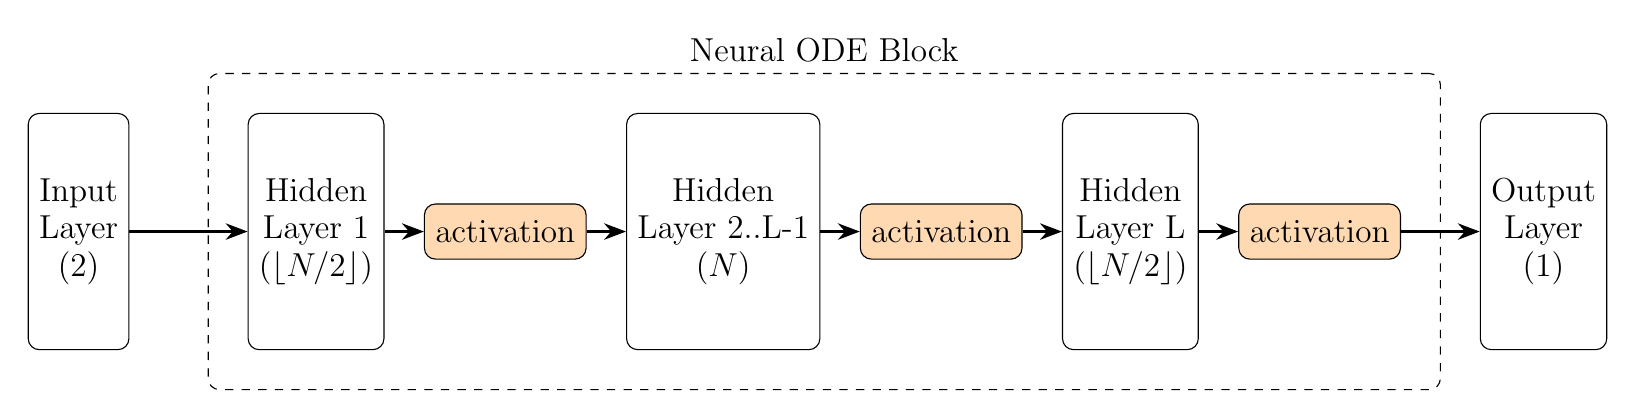
\begin{tikzpicture}[
    neuron/.style={circle, draw, minimum size=0.5cm},
    layer/.style={rectangle, draw, minimum height=3cm, rounded corners, align=center},
    arrow/.style={-{Stealth[scale=1.2]}, thick},
    activation/.style={rectangle, draw, minimum height=0.7cm, minimum width=2cm, rounded corners, fill=orange!30},
    node distance=1.5cm
    ]

    % Define the layers
    \node[layer, minimum width=1.2cm] (input) {Input\\Layer\\(2)};
    \node[layer, minimum width=1.2cm, right=of input] (h1) {Hidden\\Layer 1\\($\lfloor N/2 \rfloor$)};
    \node[activation, right=0.5cm of h1] (act1) {activation};
    \node[layer, minimum width=1.2cm, right=0.5cm of act1] (h2) {Hidden\\Layer 2..L-1\\($N$)};
    \node[activation, right=0.5cm of h2] (act2) {activation};
    \node[layer, minimum width=1.2cm, right=0.5cm of act2] (h3) {Hidden\\Layer L\\($\lfloor N/2 \rfloor$)};
    \node[activation, right=0.5cm of h3] (act3) {activation};


    \node[layer, minimum width=1.2cm, right=1cm of act3] (output) {Output\\Layer\\(1)};

    % Connect the layers
    \draw[arrow] (input) -- (h1) node[midway, above] {};
    \draw[arrow] (h1) -- (act1);
    \draw[arrow] (act1) -- (h2) node[midway, above] {};
    \draw[arrow] (h2) -- (act2);
    \draw[arrow] (act2) -- (h3) node[midway, above] {};
    \draw[arrow] (h3) -- (act3);
    \draw[arrow] (act3) -- (output) node[midway, above] {};

    % \draw[arrow] (act3) -- (h4) node[midway, above] {};
    % \draw[arrow] (h4) -- (act4);
    % \draw[arrow] (act4) -- (h5) node[midway, above] {};
    % \draw[arrow] (h5) -- (act6) node[midway, above] {};

    % \draw[arrow] (act6) -- (output) node[midway, above] {};

    % Add ODE block annotation
    \node[draw, dashed, rounded corners, fit={(h1) (h2) (h3)  (act1) (act2) (act3)}, inner sep=0.5cm, label=above:Neural ODE Block] {};

    % Add title
    % \node[above=0.7cm of input, font=\Large\bfseries, anchor=west] {Neural ODE Network Architecture};


\end{tikzpicture}

    }
    \caption{Schemat działania solvera ODE w trakcie procesu uczenia.}
    \label{fig:nn-arch}
\end{figure}

\section{Wyniki}

Przykładowe wyniki symulacji przedstawiono na Rys.~\ref{fig:sample-results} w formie wykresów porównawczych dla memrystora domieszkowanego wolframem, poddanego sinusoidalnemu pobudzeniu napięciowemu o amplitudzie 1V oraz częstotliwości 1Hz. Analiza obejmuje trzy podstawowe charakterystyki dynamiczne przebieg prądu memrystora w czasie, przebieg napięcia przyłożonego do memrystora, pętle histerezy  napięcie–prąd ($v_m - i_m$), ilustrujące nieliniową zależność między tymi wielkościami oraz właściwości pamięciowe elementu.

\newcommand{\subwidth}{0.32\linewidth}
\begin{figure}[H]
    \centering
    \begin{subfigure}[b]{\subwidth}
        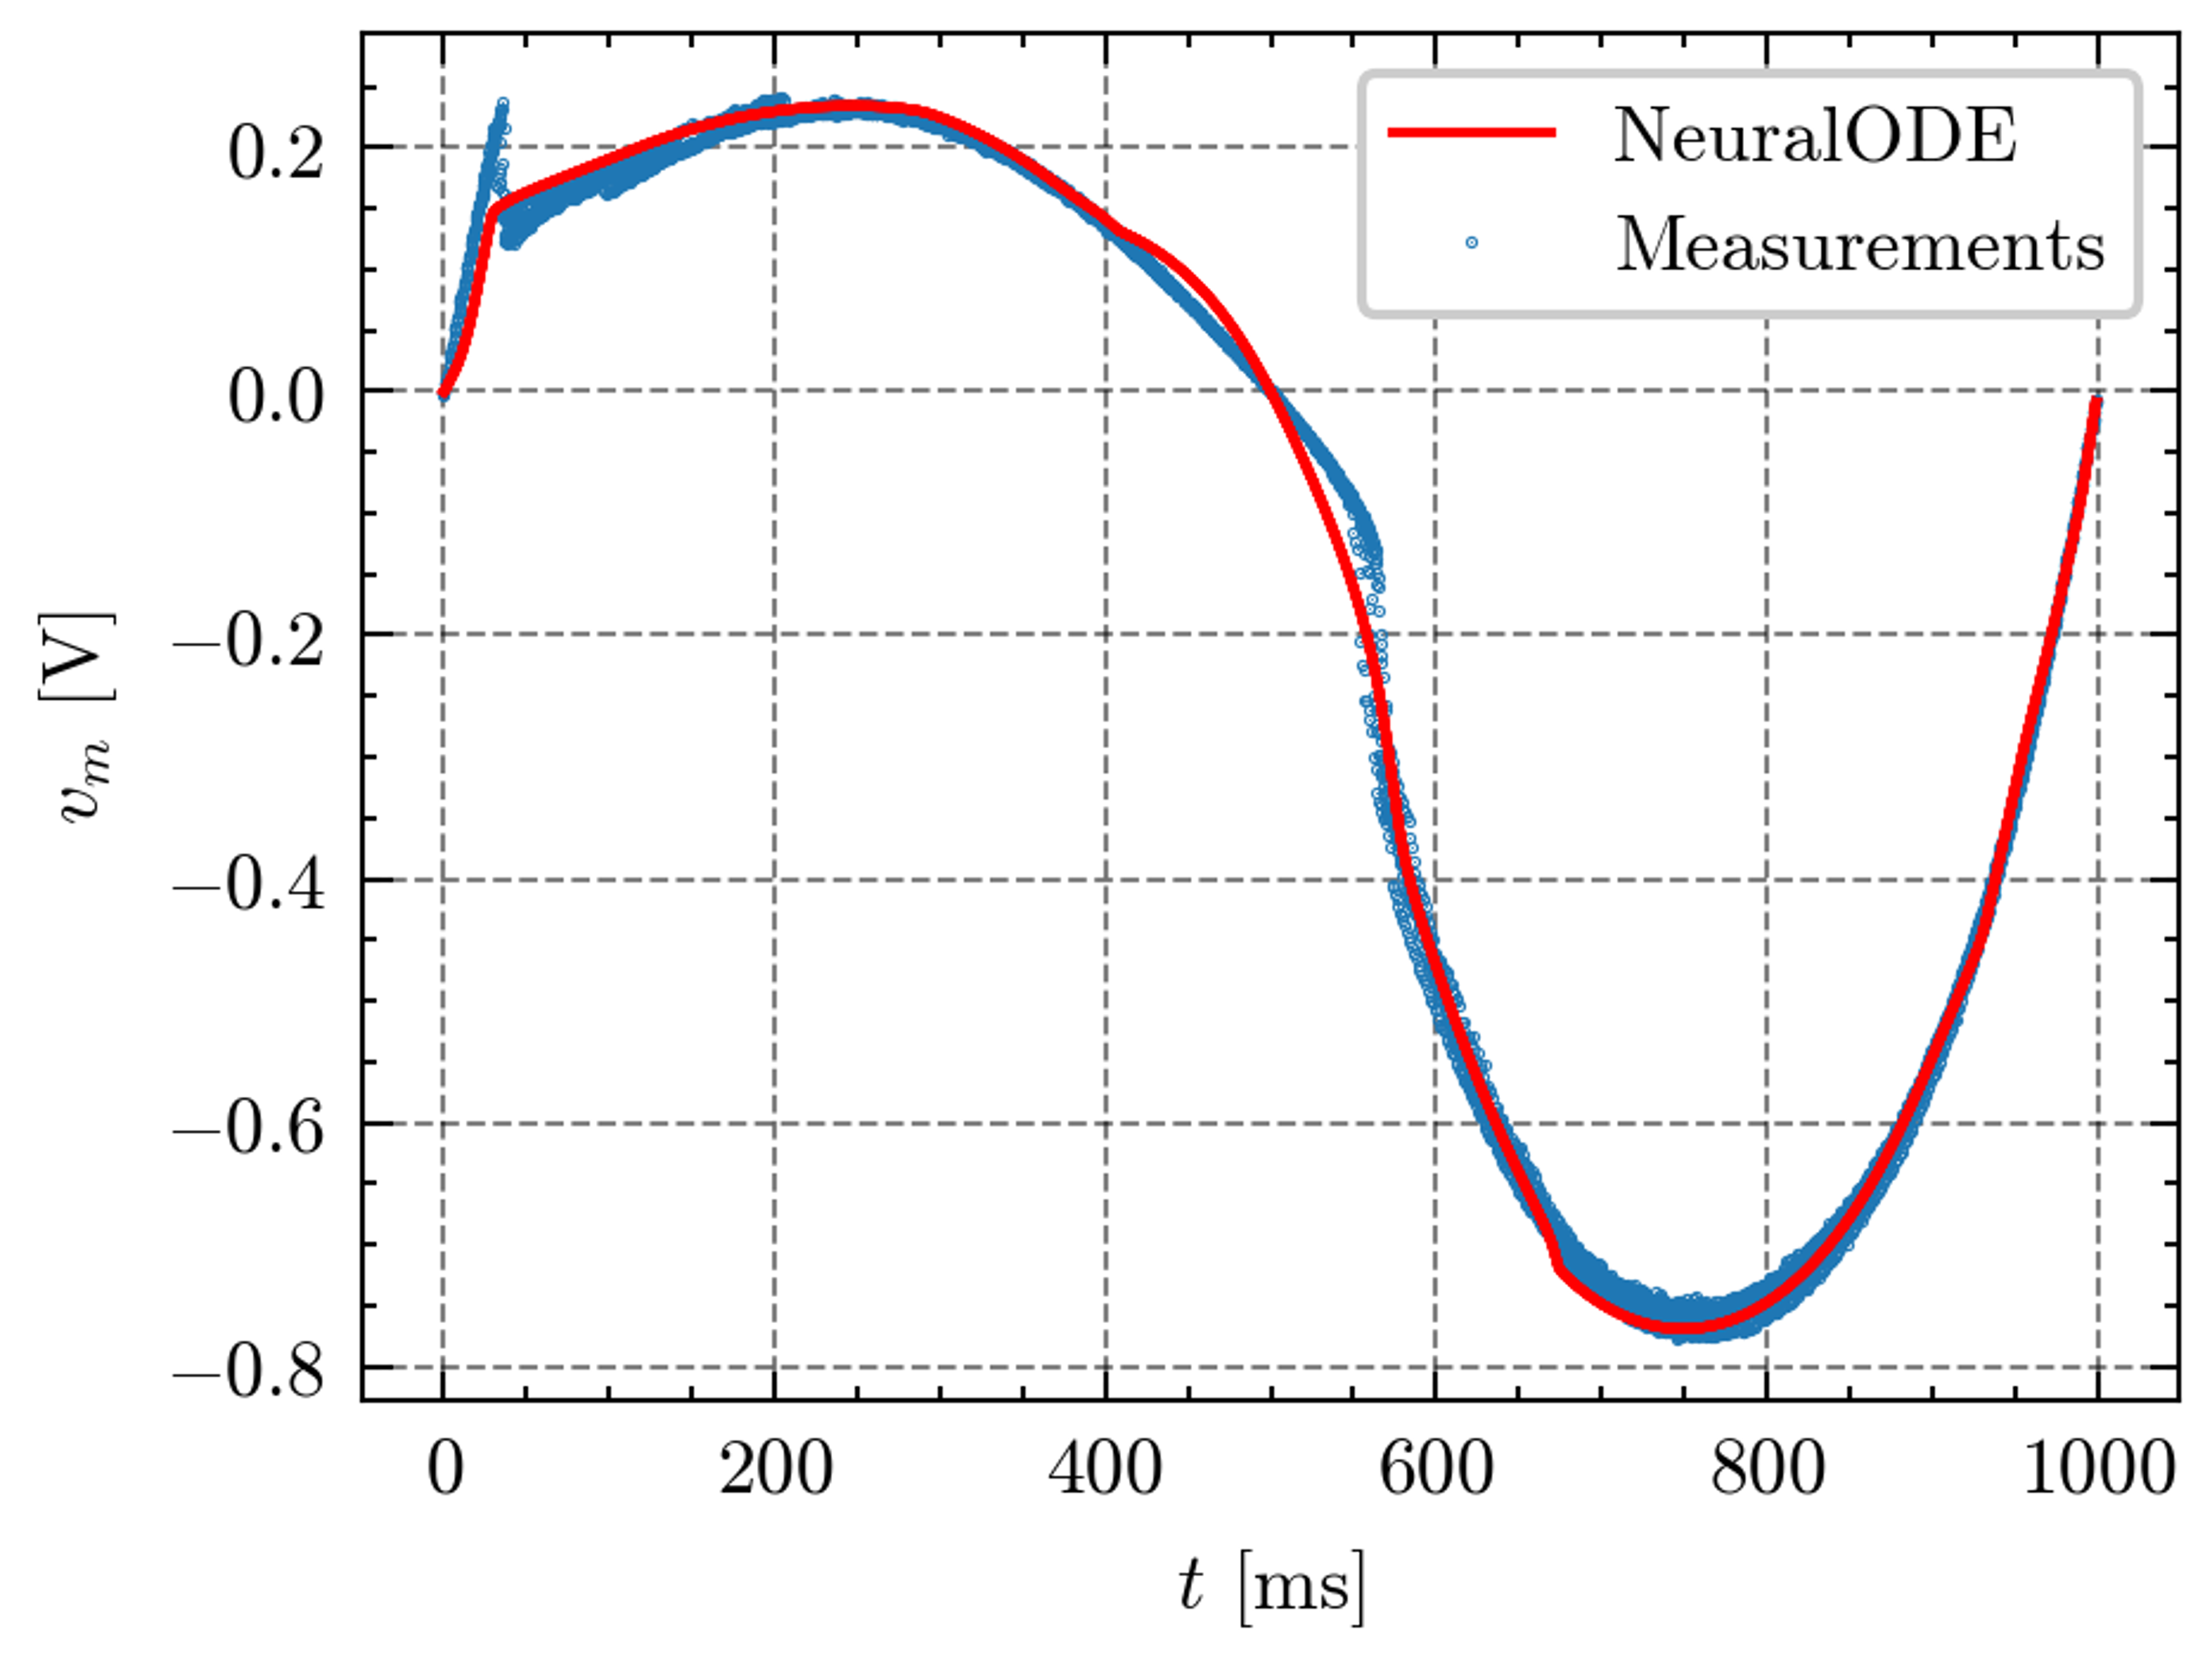
\includegraphics[width=\linewidth]{sample_results/v_m.png}
        \caption{}
    \end{subfigure}
    % \hfill
    \begin{subfigure}[b]{\subwidth}
        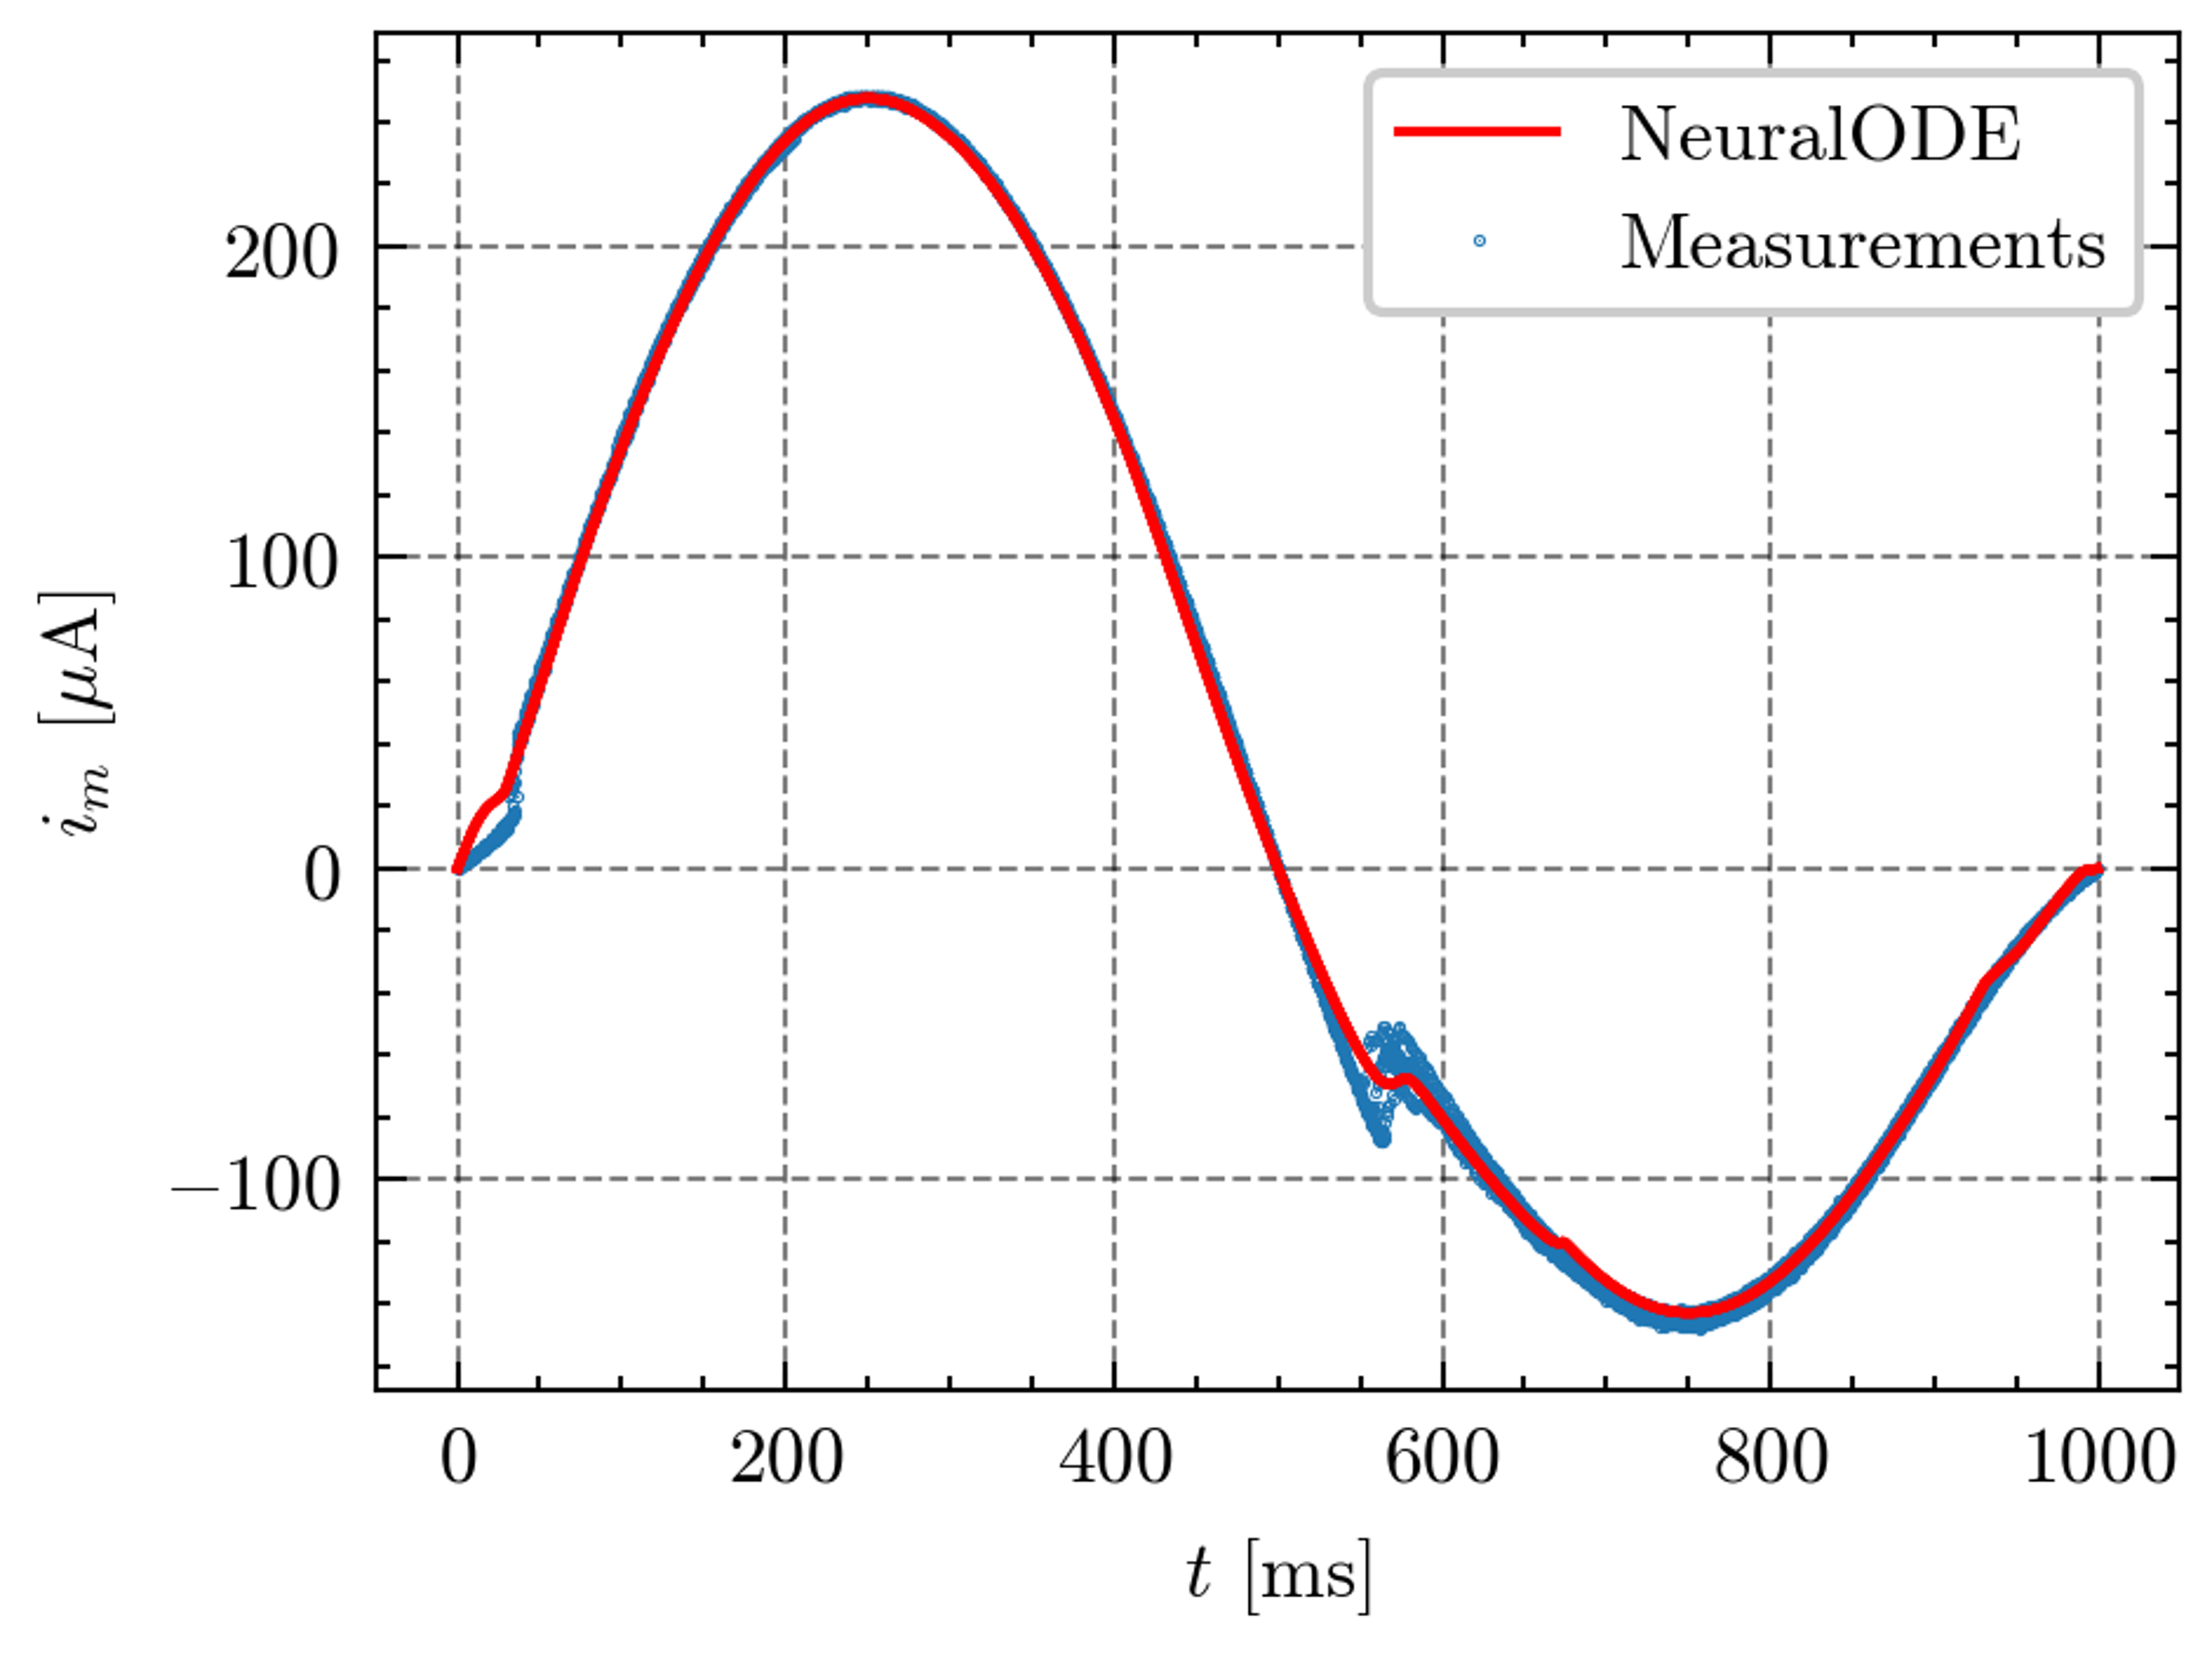
\includegraphics[width=\linewidth]{sample_results/i_m.png}
        \caption{}
    \end{subfigure}
    \begin{subfigure}[b]{\subwidth}
        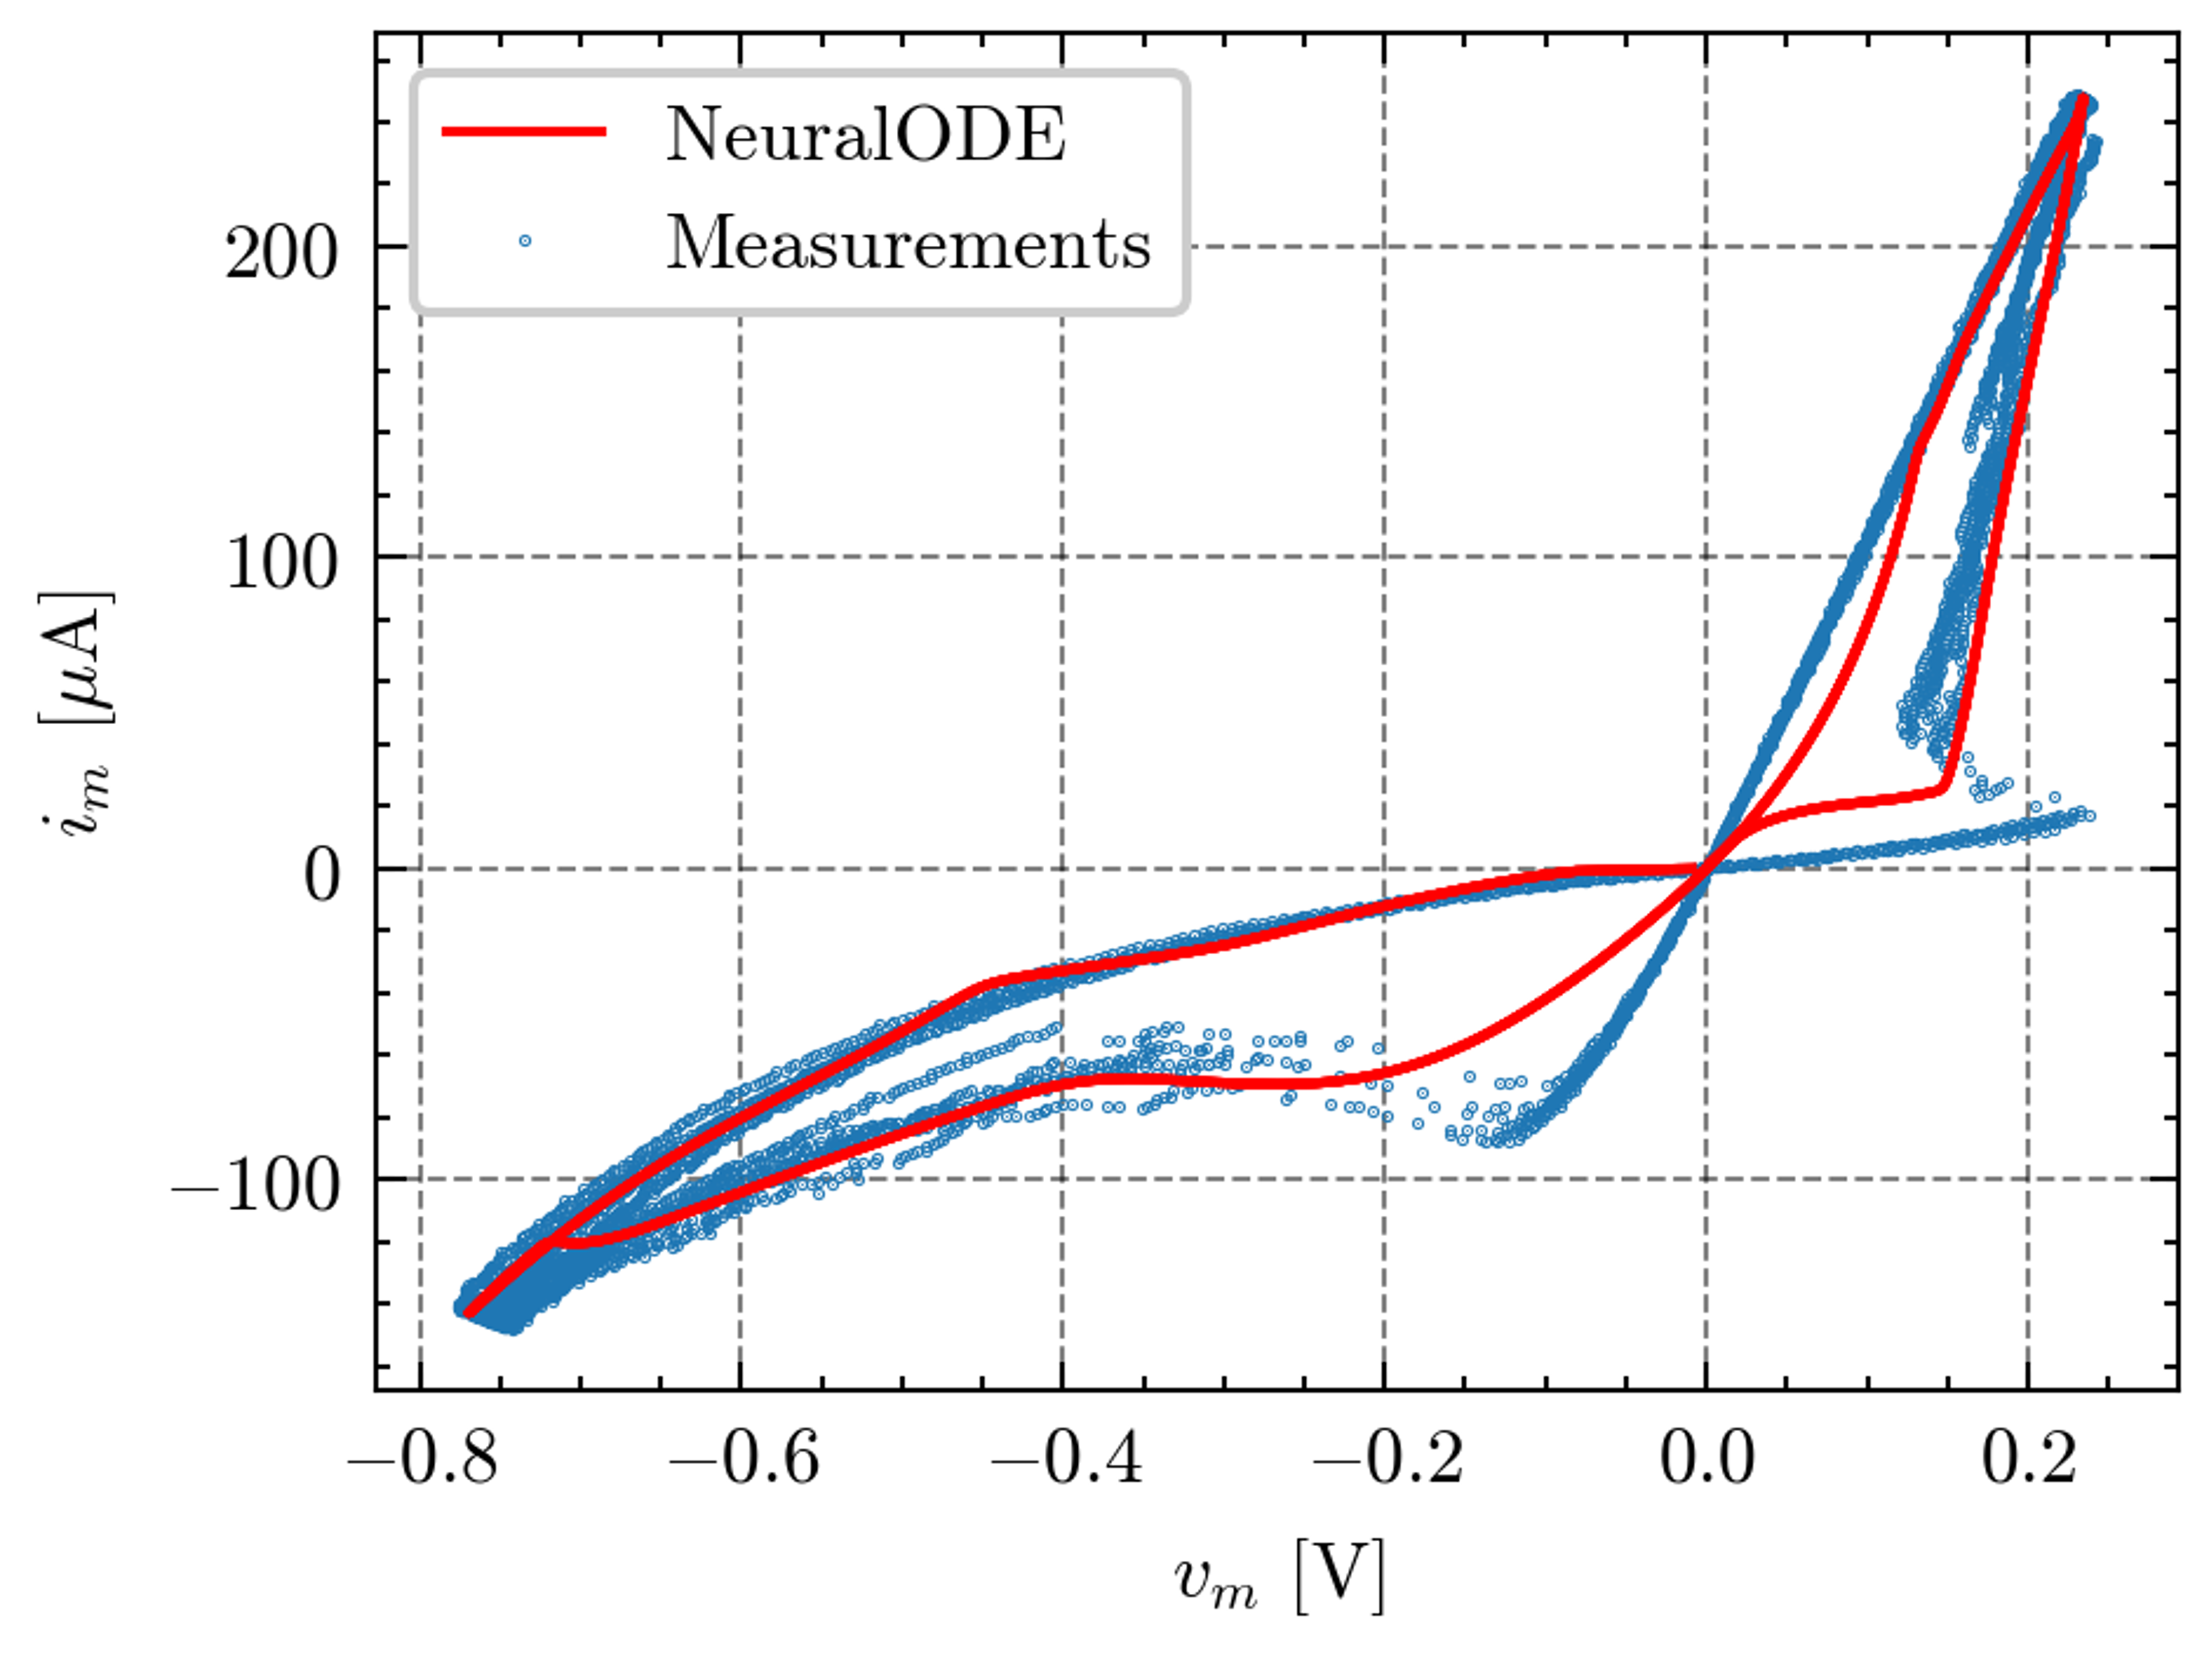
\includegraphics[width=\linewidth]{sample_results/hysteresis.png}
        \caption{}
    \end{subfigure}
    \caption{Przykładowe wyniki symulacji memrystora domieszkowanego wolframem, poddanego sinusoidalnemu pobudzeniu napięciowemu o amplitudzie 1V oraz częstotliwości 1Hz. (a) Przebieg napięcia przyłożonego do memrystora, (b) Przebieg prądu memrystora, (c) Pętla histerezy napięcie–prąd ($v_m - i_m$).}
    \label{fig:sample-results}
\end{figure}



\begin{figure}[htbp!]
    \centering
    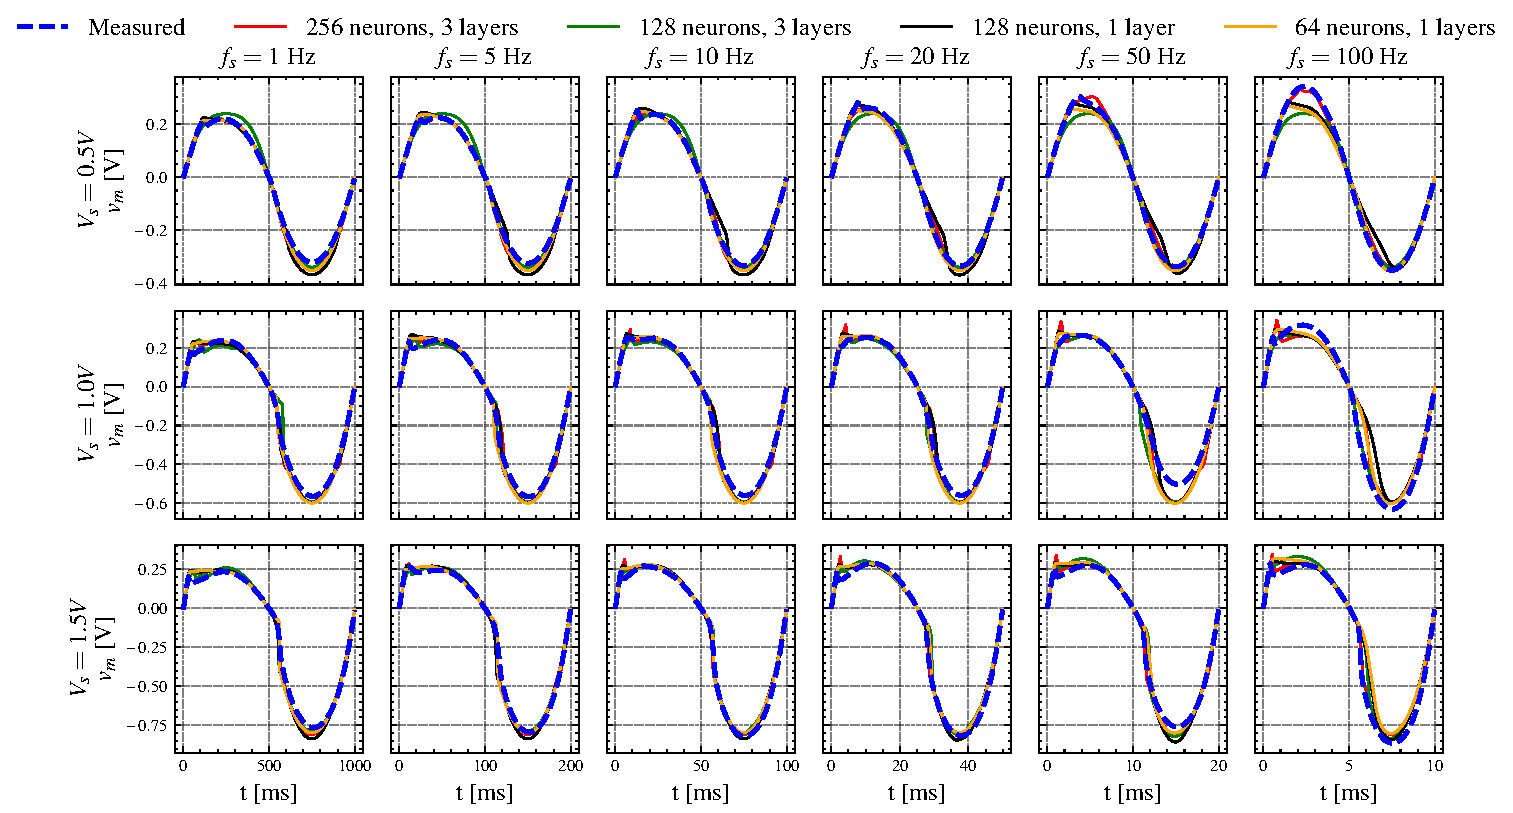
\includegraphics[width=\linewidth]{sample_results/simulated_vms.pdf}
    \caption{Porównanie uśrednionych do jednego okresu , przebiegów napięcia na memrystorze $v_m$ dla różnych architektur sieci neuronowej.}
\end{figure}

\begin{figure}[htbp!]
    \centering
    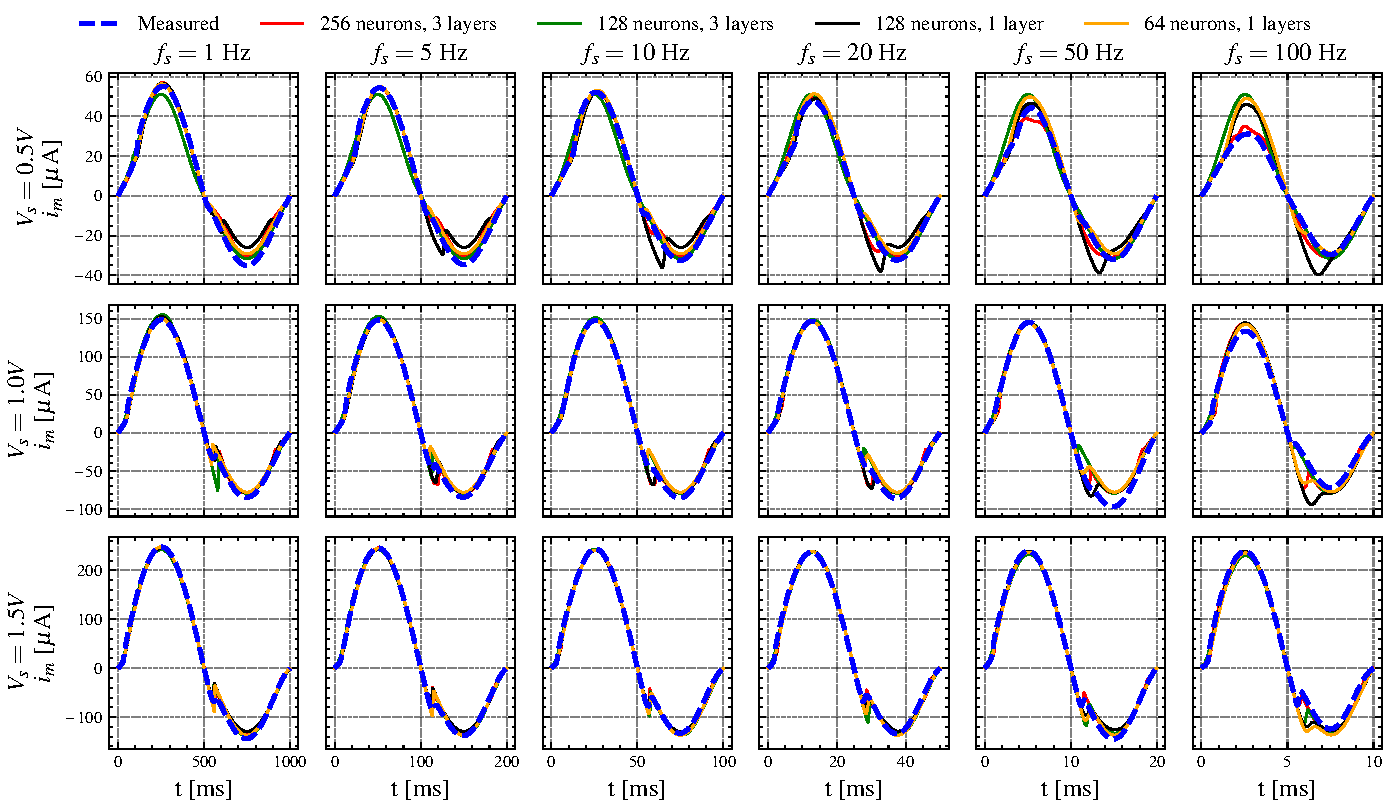
\includegraphics[width=\linewidth]{sample_results/simulated_ims.pdf}
    \caption{Porównanie uśrednionych do jednego okresu, przebiegów prądu memrystora $i_m$ dla różnych architektur sieci neuronowej.}
\end{figure}


\begin{figure}[htbp!]
    \centering
    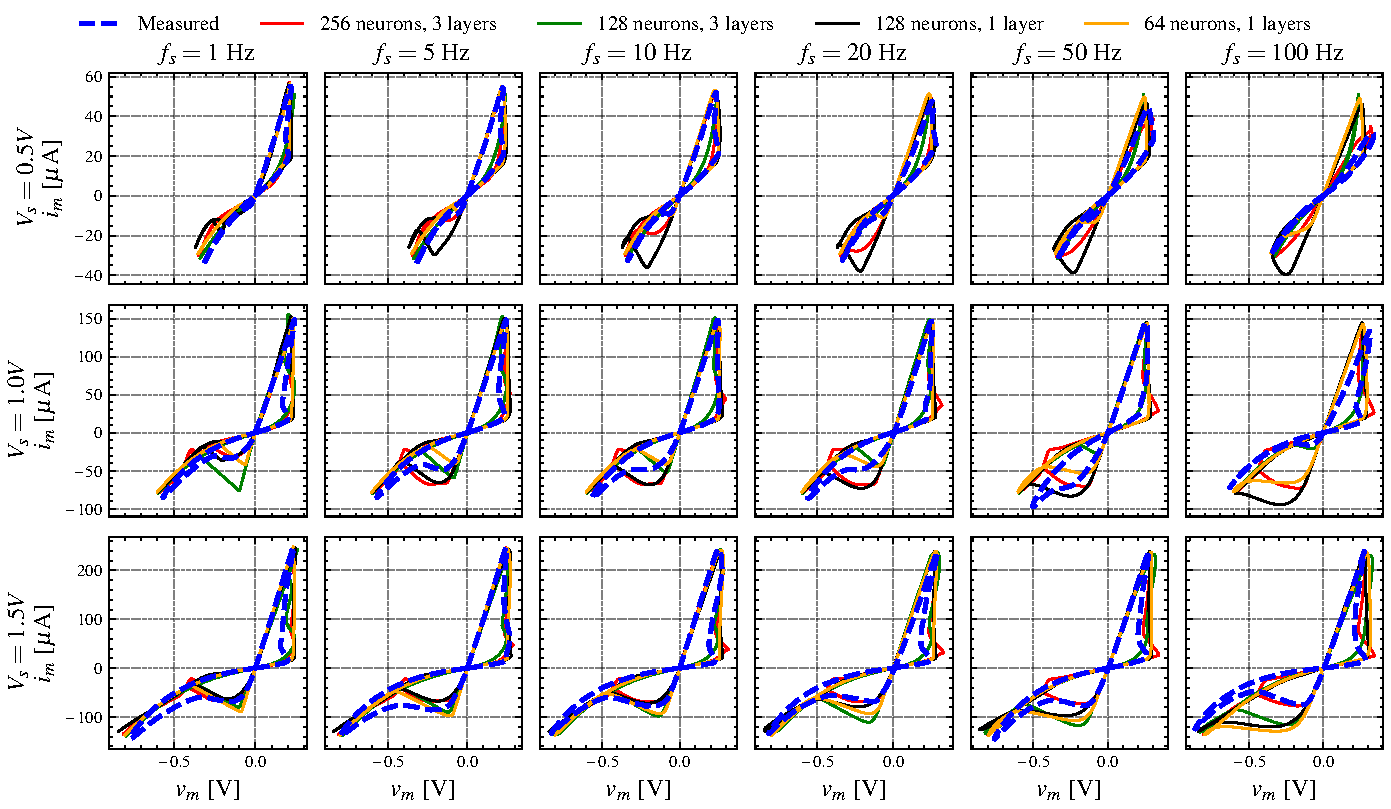
\includegraphics[width=\linewidth]{sample_results/simulated_histeresis.pdf}
    \caption{Porównanie uśrednionych do jednego okresu, pętli histerezy $v_m - i_m$ memrystora  dla różnych architektur sieci neuronowej.}
\end{figure}


\begin{figure}
    \begin{subfigure}[c]{0.48\linewidth}
        \centering
        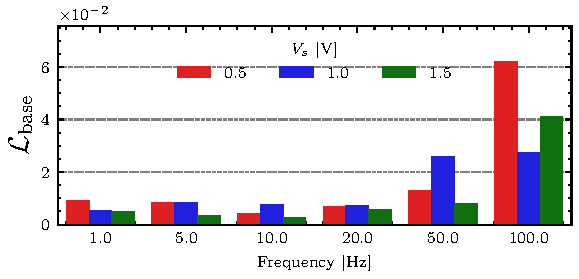
\includegraphics[width=\linewidth]{sample_results/loss_per_freq_model_silu_64_1best_cpu.pdf}
        \caption{64 neurons, 1 layer}
    \end{subfigure}
    \begin{subfigure}[c]{0.48\linewidth}
        \centering
        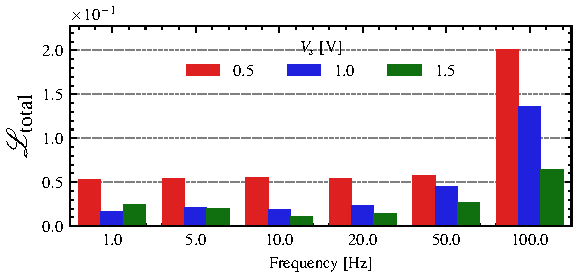
\includegraphics[width=\linewidth]{sample_results/loss_per_freq_model_silu_128_1best_cpu.pdf}
        \caption{128 neurons, 1 layer}
    \end{subfigure}
    \begin{subfigure}[c]{0.48\linewidth}
        \centering
        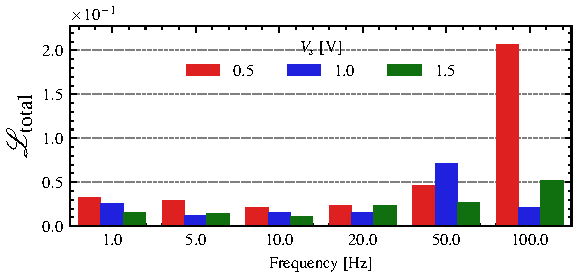
\includegraphics[width=\linewidth]{sample_results/loss_per_freq_model_silu_128_3best_cpu.pdf}
        \caption{128 neurons, 3 layers}

    \end{subfigure}
    \begin{subfigure}[c]{0.48\linewidth}
        \centering
        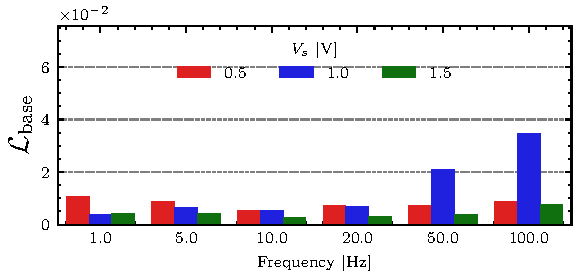
\includegraphics[width=\linewidth]{sample_results/loss_per_freq_model_silu_256_3_cpu.pdf}
        \caption{256 neurons, 3 layers}

    \end{subfigure}
    \caption{Porównanie funkcji straty dla różnych architektur sieci neuronowej.}
    \label{fig:loss_per_freq}
\end{figure}

\clearpage

\subsection{Porównanie z modelem MMS}

Porównano wyniki symulacji uzyskane z modelu sieci neuronowej z wynikami uzyskanymi z modelu Mean Metastable Switch (MMS). Analiza obejmuje przebiegi napięcia i prądu memrystora, a także pętle histerezy. Przykładowe wyniki przedstawiono na Rys.~\ref{fig:comparison_mms}. Średnia warotść funkcji straty dla modelu sieci neuronowej wynosiła $0.002052$, natomiast dla modelu MMS wynosiła $0.005589$. Wartości te wskazują na lepszą zgodność modelu sieci neuronowej z danymi eksperymentalnymi w porównaniu do modelu MMS.

\begin{figure}[httbp!]
    \begin{subfigure}[c]{0.48\linewidth}
        \centering
        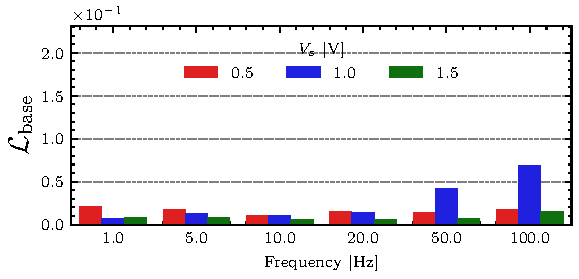
\includegraphics[width=\linewidth]{mms_results/loss_per_freq_256 neurons, 3 layers.pdf}
        \caption{256 neurons, 3 layers}
    \end{subfigure}
    \begin{subfigure}[c]{0.48\linewidth}
        \centering
        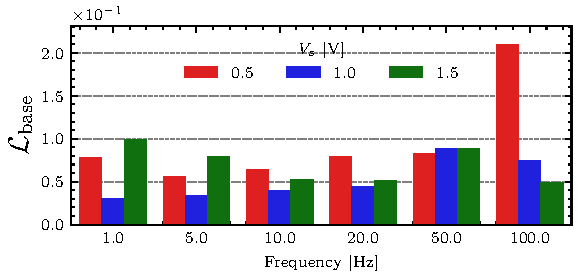
\includegraphics[width=\linewidth]{mms_results/loss_per_freq_MMS Model.pdf}
        \caption{MMS Model}
    \end{subfigure}
    \caption{Porównanie funkcji straty dla sieci neuronowej o 3 warstwach ukrytych oraz 256 neuronach (a), oraz modelu MMS (b).}
    \label{fig:comparison_mms}
\end{figure}

Przykładowe przebiegi napięcia i prądu memrystora, a także pętle histerezy dla modelu sieci neuronowej oraz modelu MMS przedstawiono na Rys.~\ref{fig:mms_vms}, \ref{fig:mms_ims}, \ref{fig:mms_histeresis}.



\begin{figure}[htbp!]
    \centering
    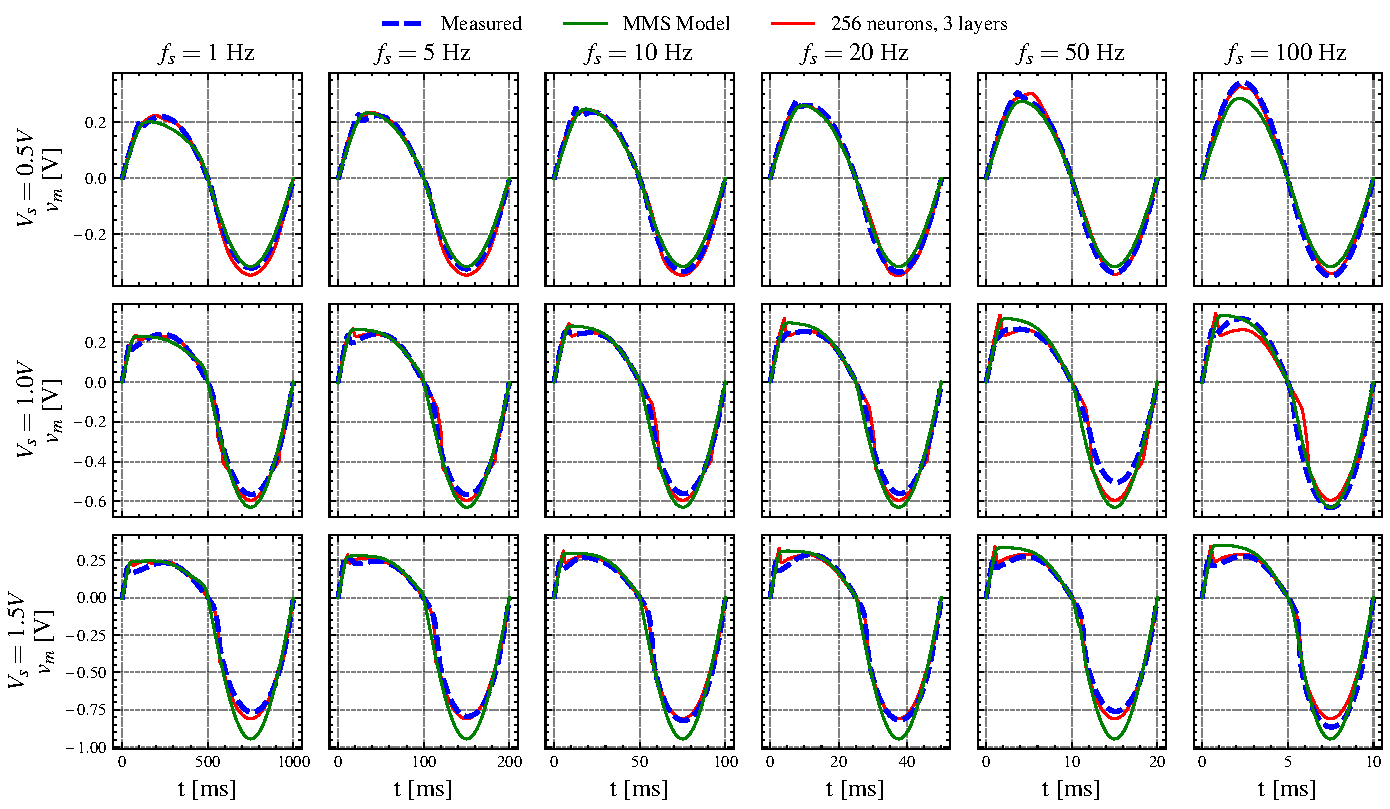
\includegraphics[width=\linewidth]{mms_results/simulated_vms.pdf}
    \caption{Porównanie uśrednionych do jednego okresu, przebiegów napięcia na memrystorze $v_m$ dla sieci neuronowej oraz modelu MMS.}
    \label{fig:mms_vms}
\end{figure}

\begin{figure}[htbp!]
    \centering
    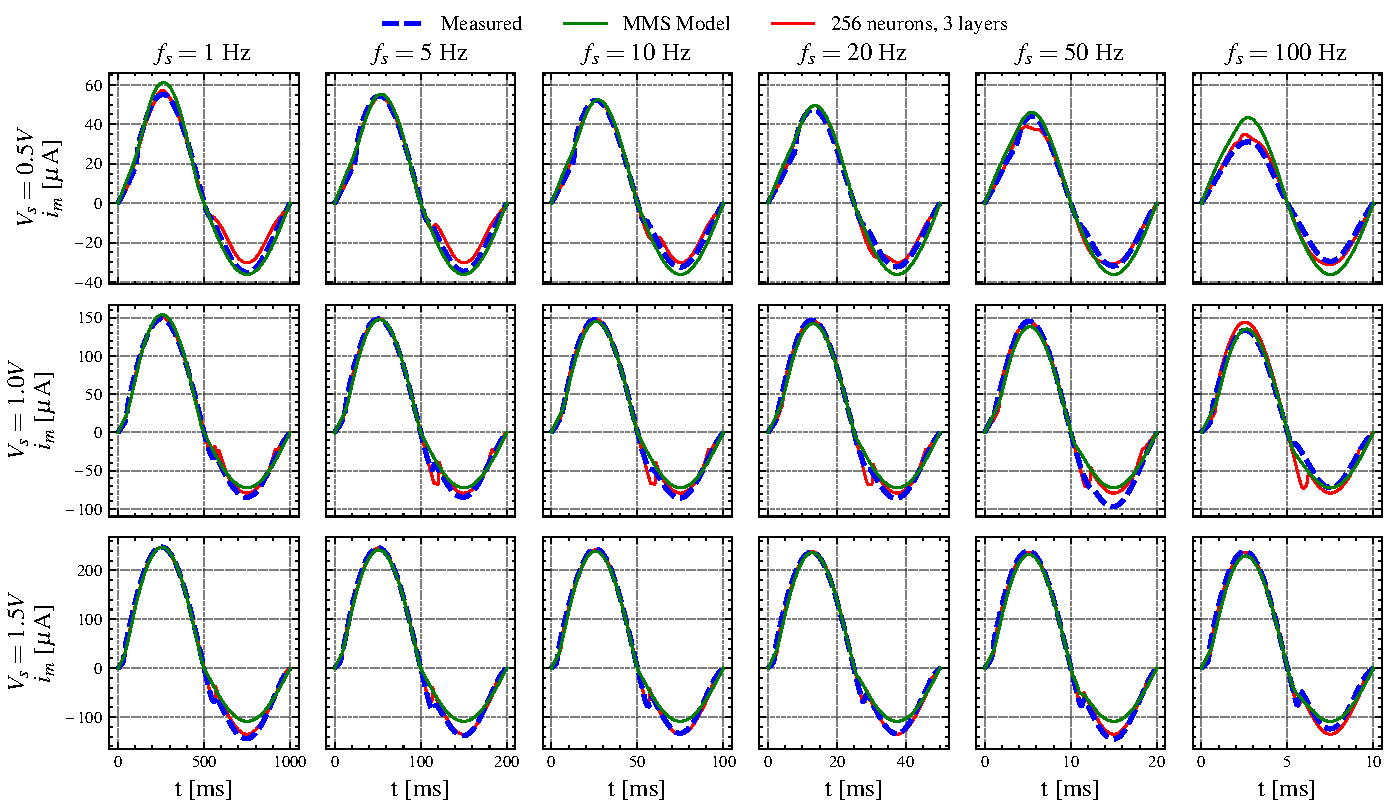
\includegraphics[width=\linewidth]{mms_results/simulated_ims.pdf}
    \caption{Porównanie uśrednionych do jednego okresu, przebiegów prądu memrystora $i_m$ dla sieci neuronowej oraz modelu MMS.}
    \label{fig:mms_ims}
\end{figure}


\begin{figure}[htbp!]
    \centering
    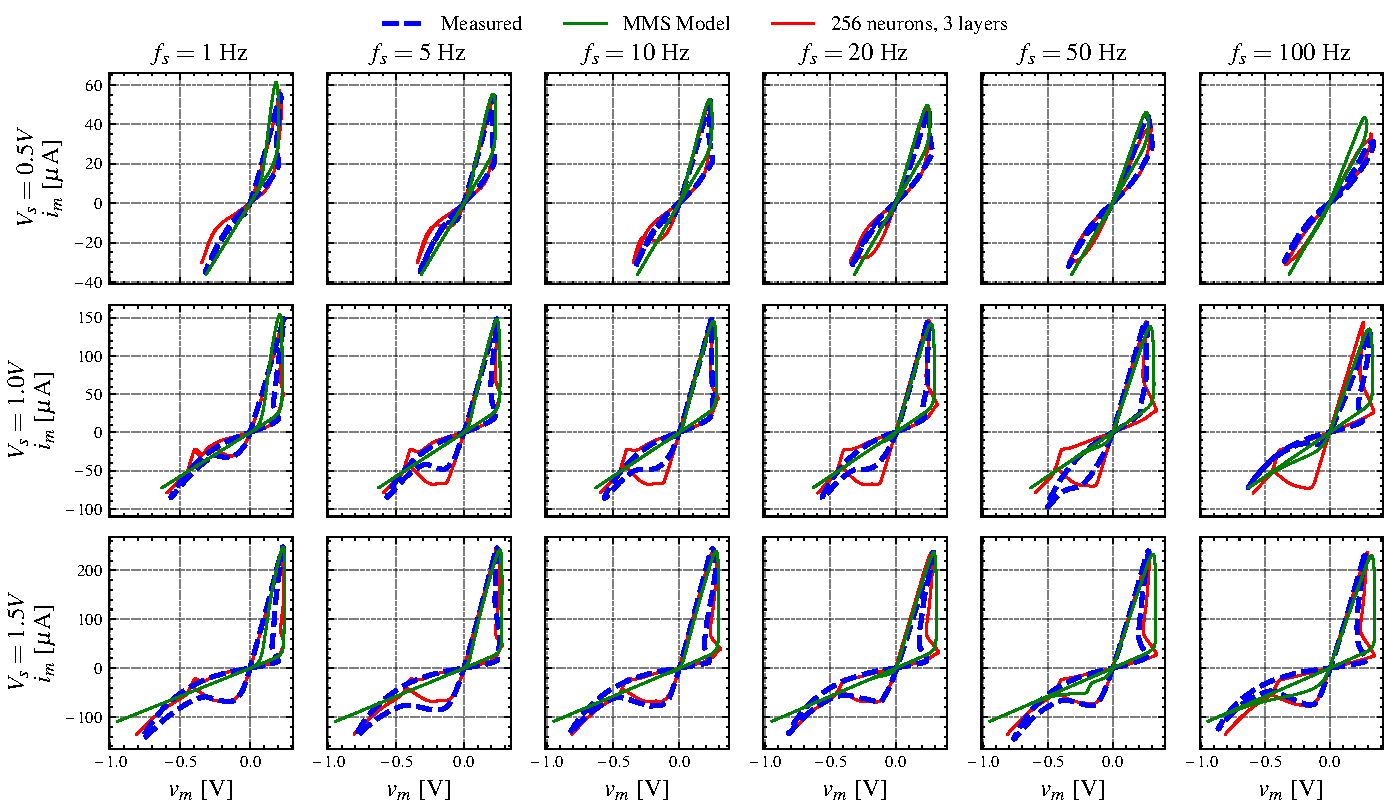
\includegraphics[width=\linewidth]{mms_results/simulated_histeresis.pdf}
    \caption{Porównanie uśrednionych do jednego okresu, pętli histerezy $v_m - i_m$ memrystora  dla sieci neuronowej oraz modelu MMS.}
    \label{fig:mms_histeresis}
\end{figure}




\subsection{Analiza wpływu hiperparametrów sieci neuronowej}
\Todo{Analiza zostanie przeprowadzona po zakończeniu procesu trenowania sieci neuronowej.}

\clearpage
\printbibliography[heading=bibintoc, title={Bibliografia}]

\end{document}
